\chapter{System Analysis and Design}
\minitoc
\clearpage
\section{Introduction}
In this chapter, we explain the analysis and design work done before coding. We describe who uses the system, how they interact with it, how data is organized, and what global architecture was chosen.

\section{Use Case Analysis}
\subsection{Actors and Access Scope}
The platform has three main actors. Each actor has a clear role in the system:

\begin{itemize}[noitemsep]
	\item \textbf{Administrator (Admin)}: manages accounts and project assignment. The Admin creates accounts, approves accounts, and assigns projects to Project Managers.
	\item \textbf{Human Resources (HR)}: works on company-wide HR follow-up. HR can view employees, employees' clock-in/out records, and employees' leave information.
	\item \textbf{Project Manager}: works at team level. The Project Manager can view members, assigned projects, and team attendance.
\end{itemize}
\newpage
\subsection{Global Use Case Diagram}


\begin{figure}[H]
	\centering
	\IfFileExists{diagrams/ch2-use-case-diagram.png}{%
		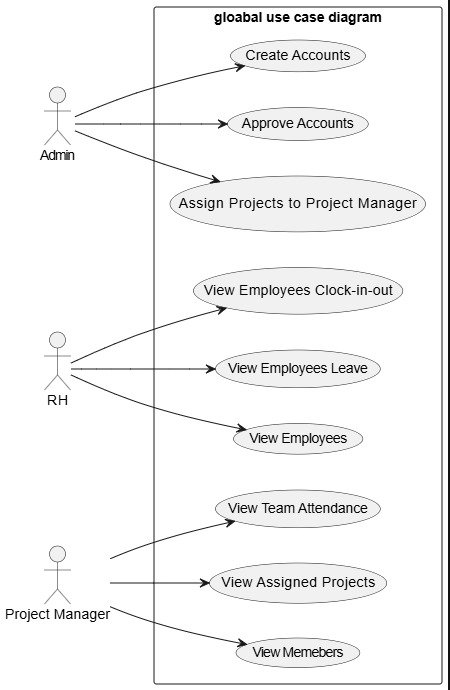
\includegraphics[width=0.86\textwidth,height=0.80\textheight,keepaspectratio]{diagrams/ch2-use-case-diagram.png}
	}{%
		\fbox{\parbox{0.9\textwidth}{
				\centering
				\vspace{2.2cm}
				\textit{Missing file: diagrams/ch2-use-case-diagram.png}\\
				\textit{Export the global use case diagram as PNG and place it in the diagrams folder.}
				\vspace{2.2cm}
		}}
	}
	\caption{Global Use Case Diagram}
	\label{fig:global-use-case}
\end{figure}

\textbf{Diagram logic (actor -- use case mapping):}
\begin{itemize}[noitemsep]
	\item \textbf{Admin}: create accounts, approve accounts, assign projects to Project Managers.
	\item \textbf{HR}: view employees, view employees' clock-in/out, view employees' leave.
	\item \textbf{Project Manager}: view members, view assigned projects, view team attendance.
\end{itemize}

\subsection{Main Use Cases Description}
\begin{center}
	\renewcommand{\arraystretch}{1.2}
	\begin{tabular}{|>{\raggedright\arraybackslash}p{3.0cm}|>{\raggedright\arraybackslash}p{4.8cm}|>{\raggedright\arraybackslash}p{6.8cm}|}
		\hline
		\textbf{Actor} & \textbf{Use Case} & \textbf{Description} \\
		\hline
		Administrator & Create Accounts & Creates HR and Project Manager accounts so users can access the platform with the right role. \\
		\hline
		Administrator & Approve Accounts & Reviews pending accounts and approves them before users can log in. \\
		\hline
		Administrator & Assign Projects to Project Manager & Assigns one or more projects to a Project Manager. \\
		\hline
		Human Resources & View Employees & Opens the employee list and checks employee information across the company. \\
		\hline
		Human Resources & View Employees Clock-in/out & Checks employee attendance records for follow-up and daily monitoring. \\
		\hline
		Human Resources & View Employees Leave & Reviews leave information to understand absences and missing attendance actions. \\
		\hline
		Project Manager & View Members & Sees the members linked to the projects under their responsibility. \\
		\hline
		Project Manager & View Assigned Projects & Sees only the projects assigned to them by the Admin. \\
		\hline
		Project Manager & View Team Attendance & Monitors the attendance of team members in assigned projects. \\
		\hline
	\end{tabular}
\end{center}

\Needspace{0.20\textheight}
\section{Data Architecture and ETL-Oriented Design}
\Needspace{0.18\textheight}
\subsection{Source Systems Exploration and Table Selection}
The two source systems, \textbf{BioTime} and \textbf{EasyProject}, contain many operational tables. To keep the integration clear and efficient, we first explored both schemas and kept only the entities needed for ETL.

\Needspace{0.76\textheight}
\vspace*{\fill}
\textbf{1) Selected BioTime Tables}
Figure~\ref{fig:biotime-selected-tables} presents the subset of tables selected from BioTime after analyzing a source schema containing roughly 200 tables. The selected tables correspond to the entities strictly required for attendance extraction, identity matching, and time-event tracking.
Figure~\ref{fig:biotime-selected-tables} shows the BioTime tables kept after the selection phase. These tables are the ones needed for attendance extraction, identity matching, and event tracking.
\begin{figure}[H]
	\centering
	\IfFileExists{diagrams/ch2-biotime-selected-tables.png}{%
		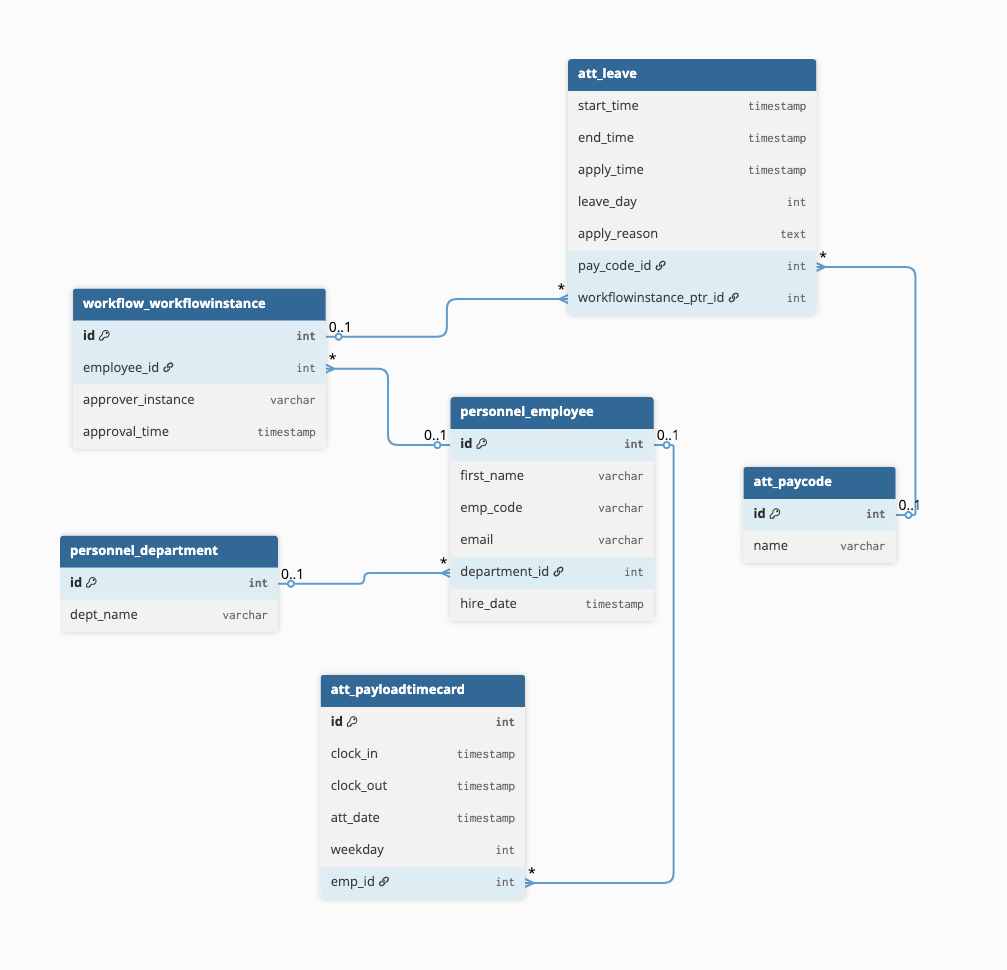
\includegraphics[width=0.96\textwidth,height=0.66\textheight,keepaspectratio]{diagrams/ch2-biotime-selected-tables.png}
	}{%
		\fbox{\parbox{0.9\textwidth}{
				\centering
				\vspace{1.8cm}
				\textit{Missing file: diagrams/ch2-biotime-selected-tables.png}\\
				\textit{Insert image of selected BioTime tables used in ETL.}
				\vspace{1.8cm}
		}}
	}
	\caption{Selected Tables from BioTime}
	\label{fig:biotime-selected-tables}
\end{figure}
\vspace*{\fill}
\clearpage

\Needspace{0.76\textheight}
\vspace*{\fill}
\textbf{2) Selected EasyProject Tables}
Figure~\ref{fig:easyproject-selected-tables} shows the EasyProject tables kept for integration. The focus was on employee data, organization structure, project assignment, and leave information used during transformation.
\begin{figure}[H]
	\centering
	\IfFileExists{diagrams/ch2-easyproject-selected-tables.png}{%
		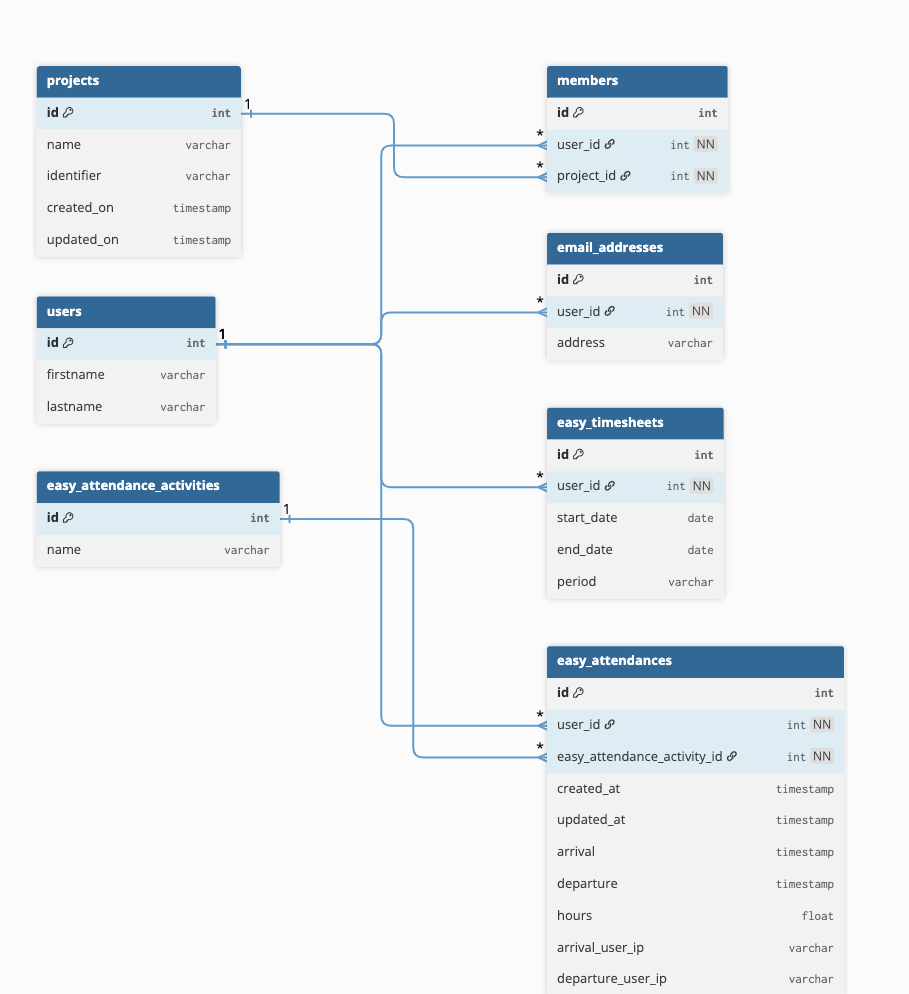
\includegraphics[width=0.96\textwidth,height=0.66\textheight,keepaspectratio]{diagrams/ch2-easyproject-selected-tables.png}
	}{%
		\fbox{\parbox{0.9\textwidth}{
				\centering
				\vspace{1.8cm}
				\textit{Missing file: diagrams/ch2-easyproject-selected-tables.png}\\
				\textit{Insert image of selected EasyProject tables used in ETL.}
				\vspace{1.8cm}
		}}
	}
	\caption{Selected Tables from EasyProject}
	\label{fig:easyproject-selected-tables}
\end{figure}
\vspace*{\fill}
\clearpage

\Needspace{0.18\textheight}
\subsection{View Layer for ETL Simplification}
After selecting the source tables, we created SQL views in each system. These views standardize field names, reduce join complexity, and provide clean ETL inputs.

\Needspace{0.74\textheight}
\vspace*{\fill}
\textbf{3) BioTime Views Created After Table Selection}
Figure~\ref{fig:biotime-created-views} illustrates the BioTime view layer. It isolates useful attendance data and gives a stable extraction interface for ETL.
\begin{figure}[H]
	\centering
	\IfFileExists{diagrams/ch2-biotime-created-views.png}{%
		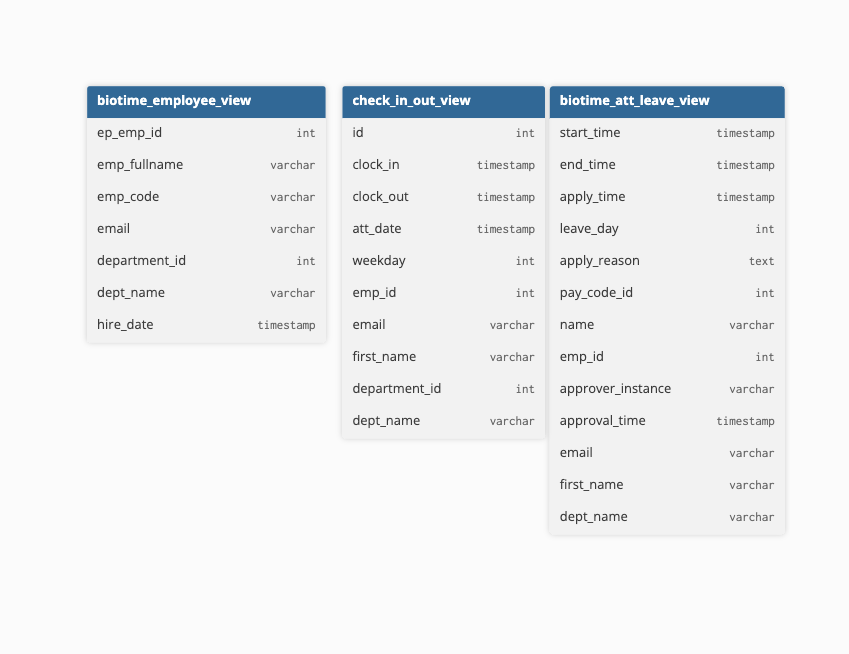
\includegraphics[width=0.96\textwidth,height=0.64\textheight,keepaspectratio]{diagrams/ch2-biotime-created-views.png}
	}{%
		\fbox{\parbox{0.9\textwidth}{
				\centering
				\vspace{1.8cm}
				\textit{Missing file: diagrams/ch2-biotime-created-views.png}\\
				\textit{Insert image of BioTime views created for ETL simplification.}
				\vspace{1.8cm}
		}}
	}
	\caption{Views Created from BioTime Selected Tables}
	\label{fig:biotime-created-views}
\end{figure}
\vspace*{\fill}
\clearpage

\Needspace{0.74\textheight}
\vspace*{\fill}
\textbf{4) EasyProject Views Created After Table Selection}
Figure~\ref{fig:easyproject-created-views} presents the EasyProject views. This intermediate layer simplifies access to HR and project attributes and harmonizes data before loading.
\begin{figure}[H]
	\centering
	\IfFileExists{diagrams/ch2-easyproject-created-views.png}{%
		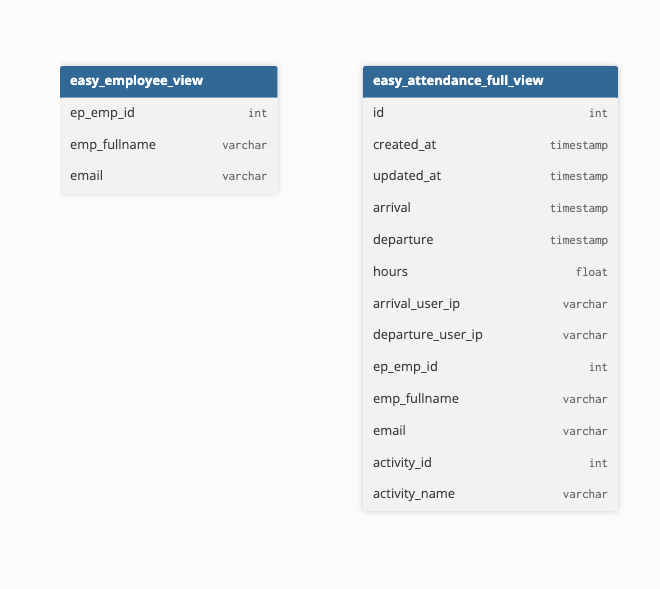
\includegraphics[width=0.96\textwidth,height=0.64\textheight,keepaspectratio]{diagrams/ch2-easyproject-created-views.png}
	}{%
		\fbox{\parbox{0.9\textwidth}{
				\centering
				\vspace{1.8cm}
				\textit{Missing file: diagrams/ch2-easyproject-created-views.png}\\
				\textit{Insert image of EasyProject views created for ETL simplification.}
				\vspace{1.8cm}
		}}
	}
	\caption{Views Created from EasyProject Selected Tables}
	\label{fig:easyproject-created-views}
\end{figure}
\vspace*{\fill}
\clearpage

\Needspace{0.16\textheight}
\subsection{Unified PostgreSQL Target Schema and Integration Constraints}
The transformed outputs from both view layers are loaded into one unified PostgreSQL schema. At this stage, identifiers and timestamps are normalized, duplicates are removed, and integrity constraints are applied to keep analytics consistent across systems.

\Needspace{0.82\textheight}
\vspace*{\fill}
\textbf{Main Application Diagram (Global Architecture Placeholder)}
Figure~\ref{fig:main-app-diagram} summarizes the main structure of the application. It shows how data moves from source systems to ETL, then to the unified database, backend services, and user modules.
\begin{figure}[H]
	\centering
	\IfFileExists{diagrams/ch2-main-app-diagram.png}{%
		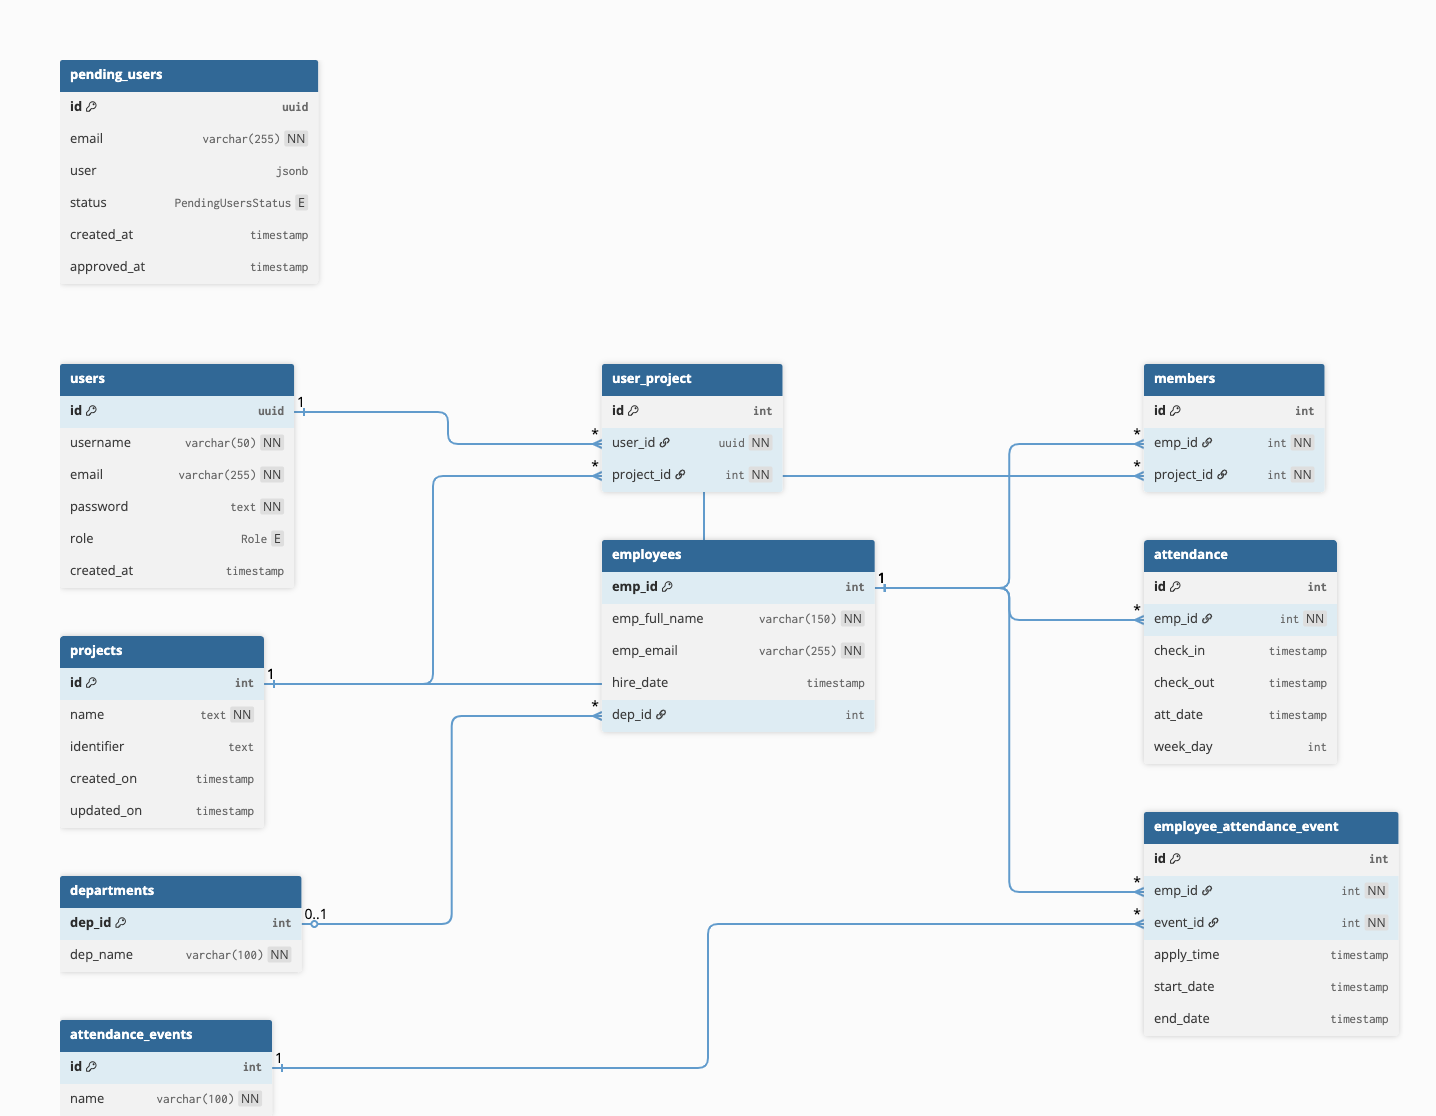
\includegraphics[width=0.98\textwidth,height=0.72\textheight,keepaspectratio]{diagrams/ch2-main-app-diagram.png}
	}{%
		\fbox{\parbox{0.9\textwidth}{
				\centering
				\vspace{2.0cm}
				\textit{Missing file: diagrams/ch2-main-app-diagram.png}\\
				\textit{Insert the main application diagram (global system view).}
				\vspace{2.0cm}
		}}
	}
	\caption{Main Application Diagram}
	\label{fig:main-app-diagram}
\end{figure}
\vspace*{\fill}
\clearpage

\Needspace{0.20\textheight}
\section{Global System Architecture}

The architecture starts by extracting data from \textbf{BioTime (PostgreSQL)} and \textbf{EasyProject (MySQL)} with \textbf{SQLAlchemy}. The data is then transformed and loaded into the main application database.

On top of this unified database, the backend uses \textbf{FastAPI}, \textbf{Alembic}, and \textbf{SQLAlchemy}. It exposes endpoints consumed by a frontend built with \textbf{React}, \textbf{Tailwind CSS}, and \textbf{shadcn/ui}.

\Needspace{0.70\textheight}
\vspace*{\fill}
\textbf{Global System Architecture Diagram}
Figure~\ref{fig:global-system-architecture} presents the end-to-end architecture, from source systems and ETL processing to the unified database, backend services, and frontend modules.

\begin{figure}[H]
	\centering
	\IfFileExists{diagrams/ch2-global-system-architecture.png}{%
		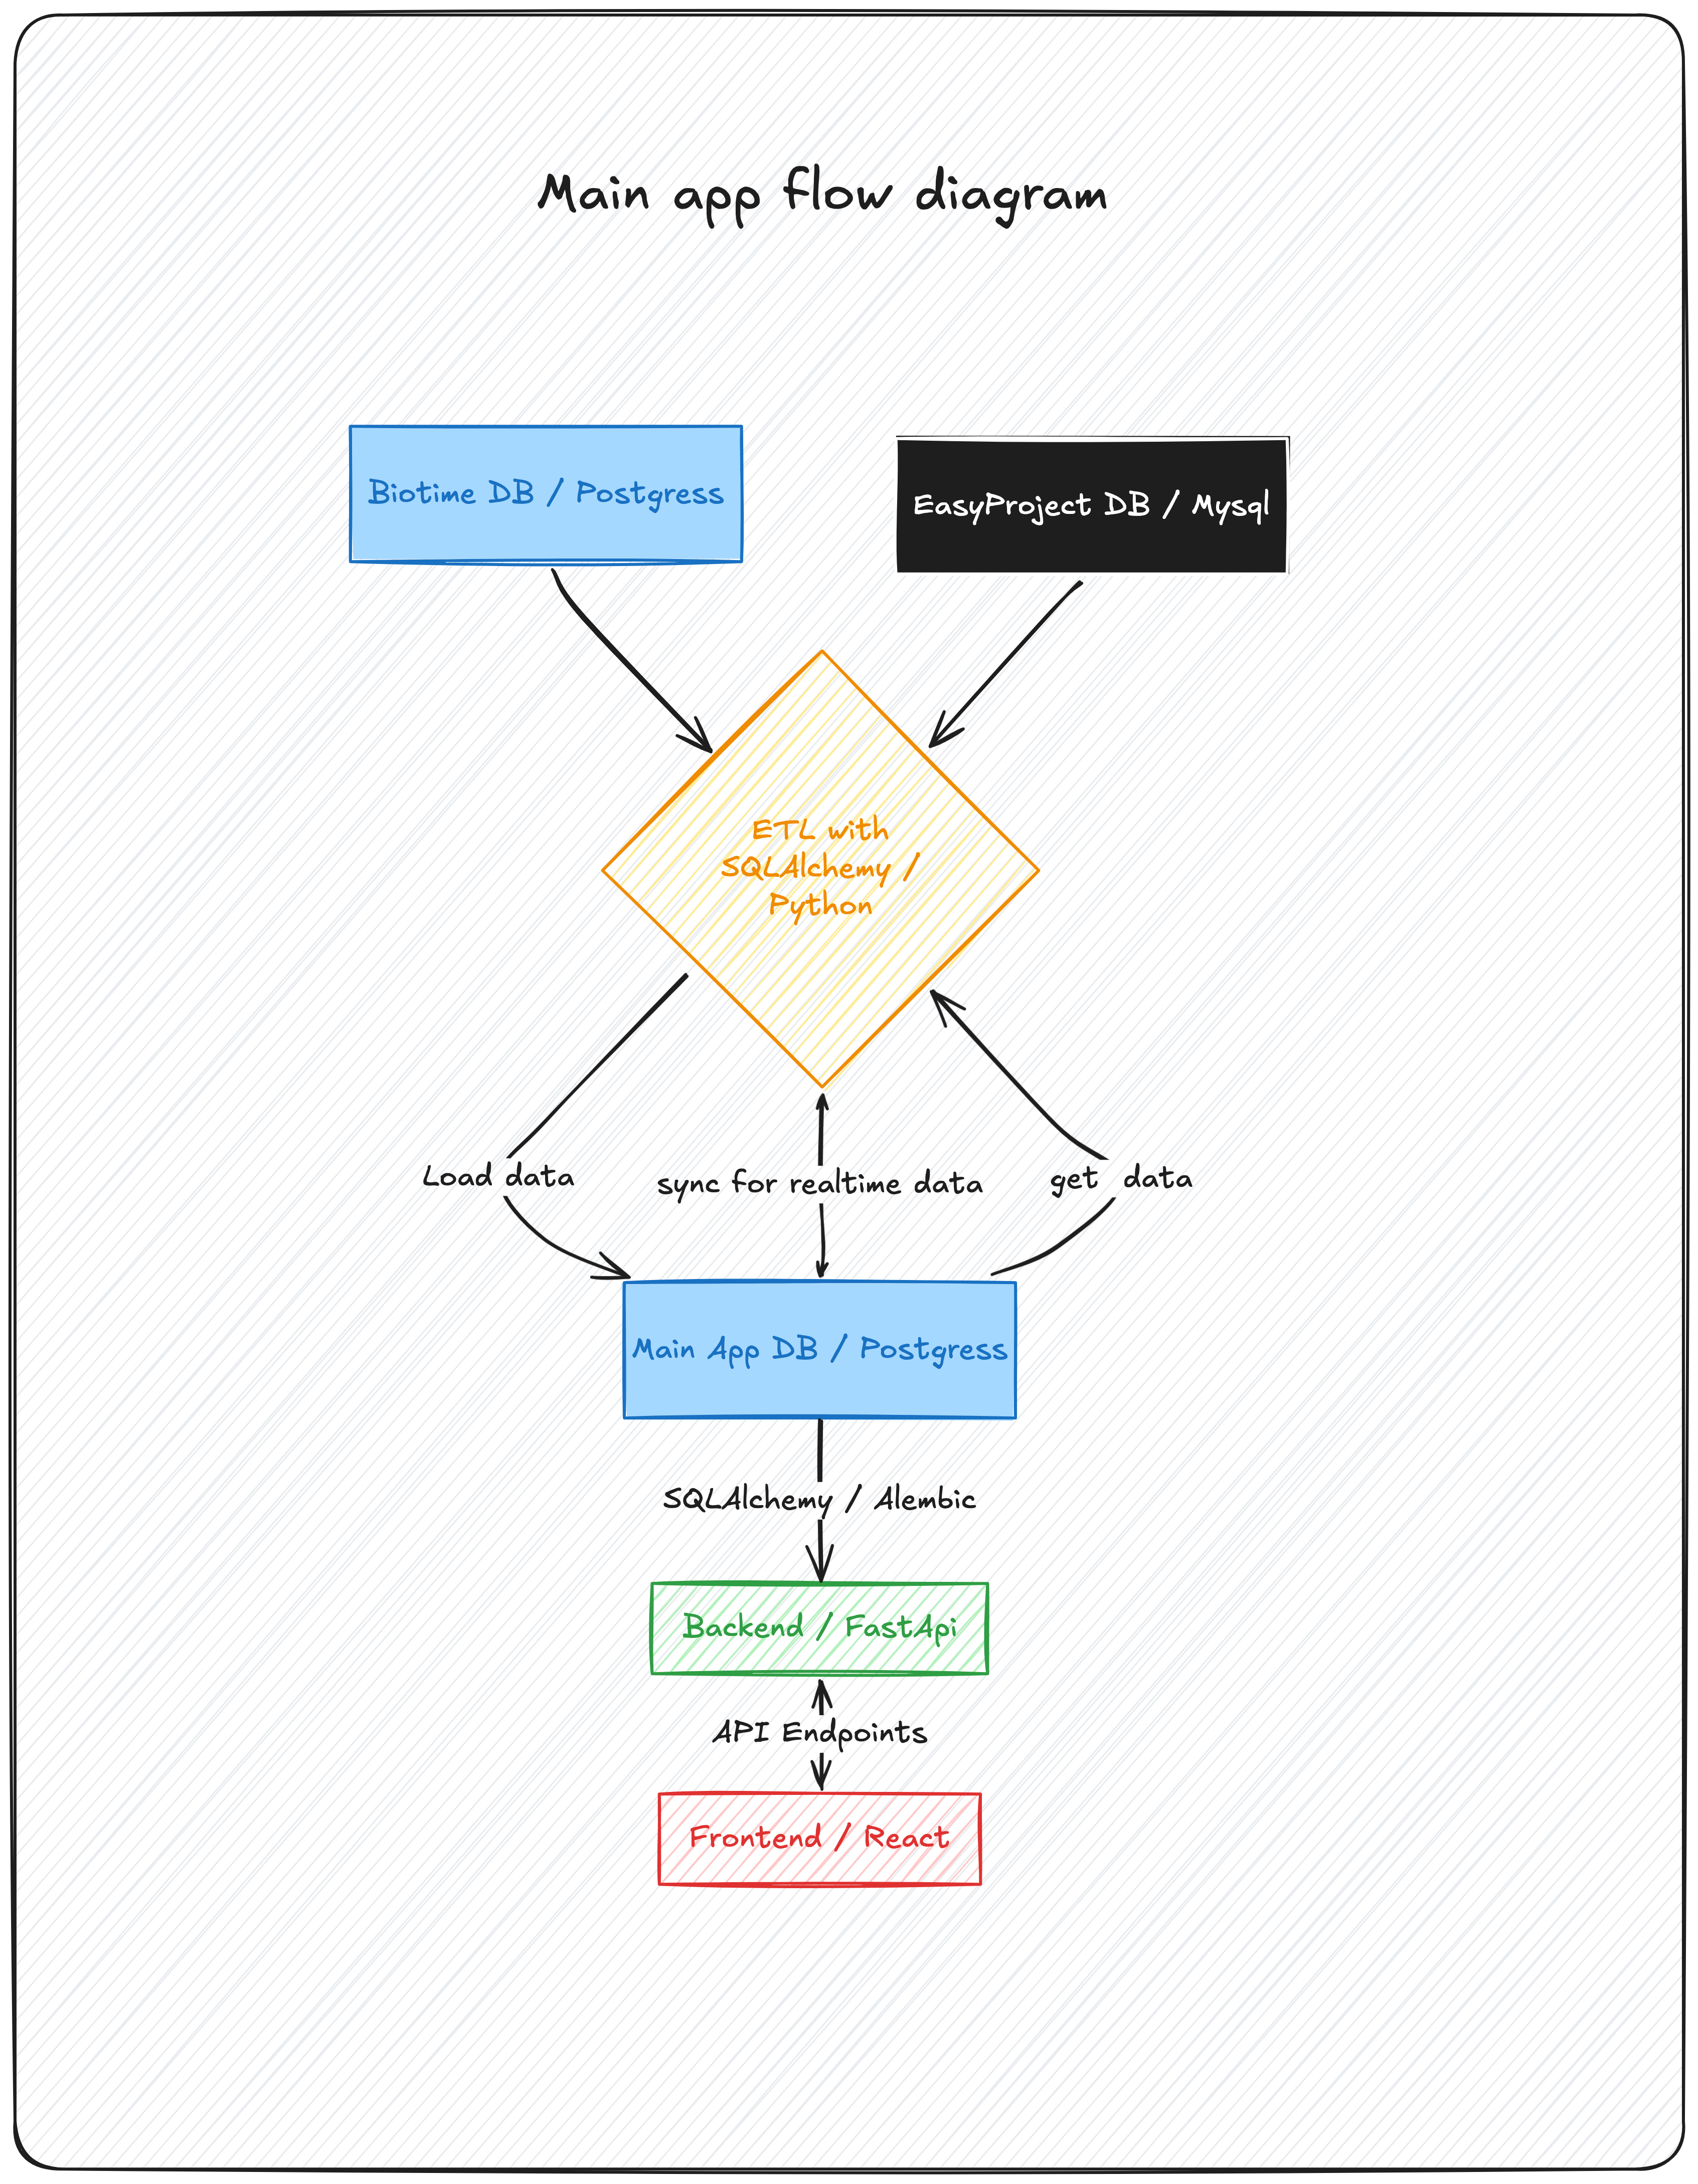
\includegraphics[width=0.98\textwidth,height=0.72\textheight,keepaspectratio]{diagrams/ch2-global-system-architecture.png}
	}{%
		\fbox{\parbox{0.9\textwidth}{
				\centering
				\vspace{2.0cm}
				\textit{Missing file: diagrams/ch2-global-system-architecture.png}\\
				\textit{Insert the global system architecture flow diagram.}
				\vspace{2.0cm}
		}}
	}
	\caption{Global System Architecture Flow}
	\label{fig:global-system-architecture}
\end{figure}



\section{Chapter Conclusion}
This chapter explained the analysis and design choices of the solution. It covered actors and use cases, ETL-focused data architecture decisions, and the global system architecture. The next chapter focuses on authentication architecture and workflows.
